\section{Number Theoretic Functions}
\epigraph{\emph{No one has yet discovered any warlike purpose to be served by the theory of numbers or relativity, and it seems unlikely that anyone will do so for many years.}}
{---G.\xspace H.\xspace Hardy}

\noindent
Number Theory is the branch of mathematics that studies the nature
and properties of numbers. Though many have made important contributions
to the field, including Gau{\ss} in his \emph{Disquisitiones
Arithmeticae} (which he completed when he was 21 years old), the
most important for public-key cryptography are Fermat and Euler
(Figure\xspace\ref{fig:euler}).

You will first need to implement the functions that drive the
mathematics behind SS before you can tackle your SS library. The
interface for these functions will be given in \texttt{numtheory.h} and
should be defined in corresponding \textbf{C} file. Read each of the subsections
carefully to understand, on some level, the theory behind each of the
number theoretic functions. Pseudocode is provided to assist you.

\begin{figure}[tbhp]
        \centering
        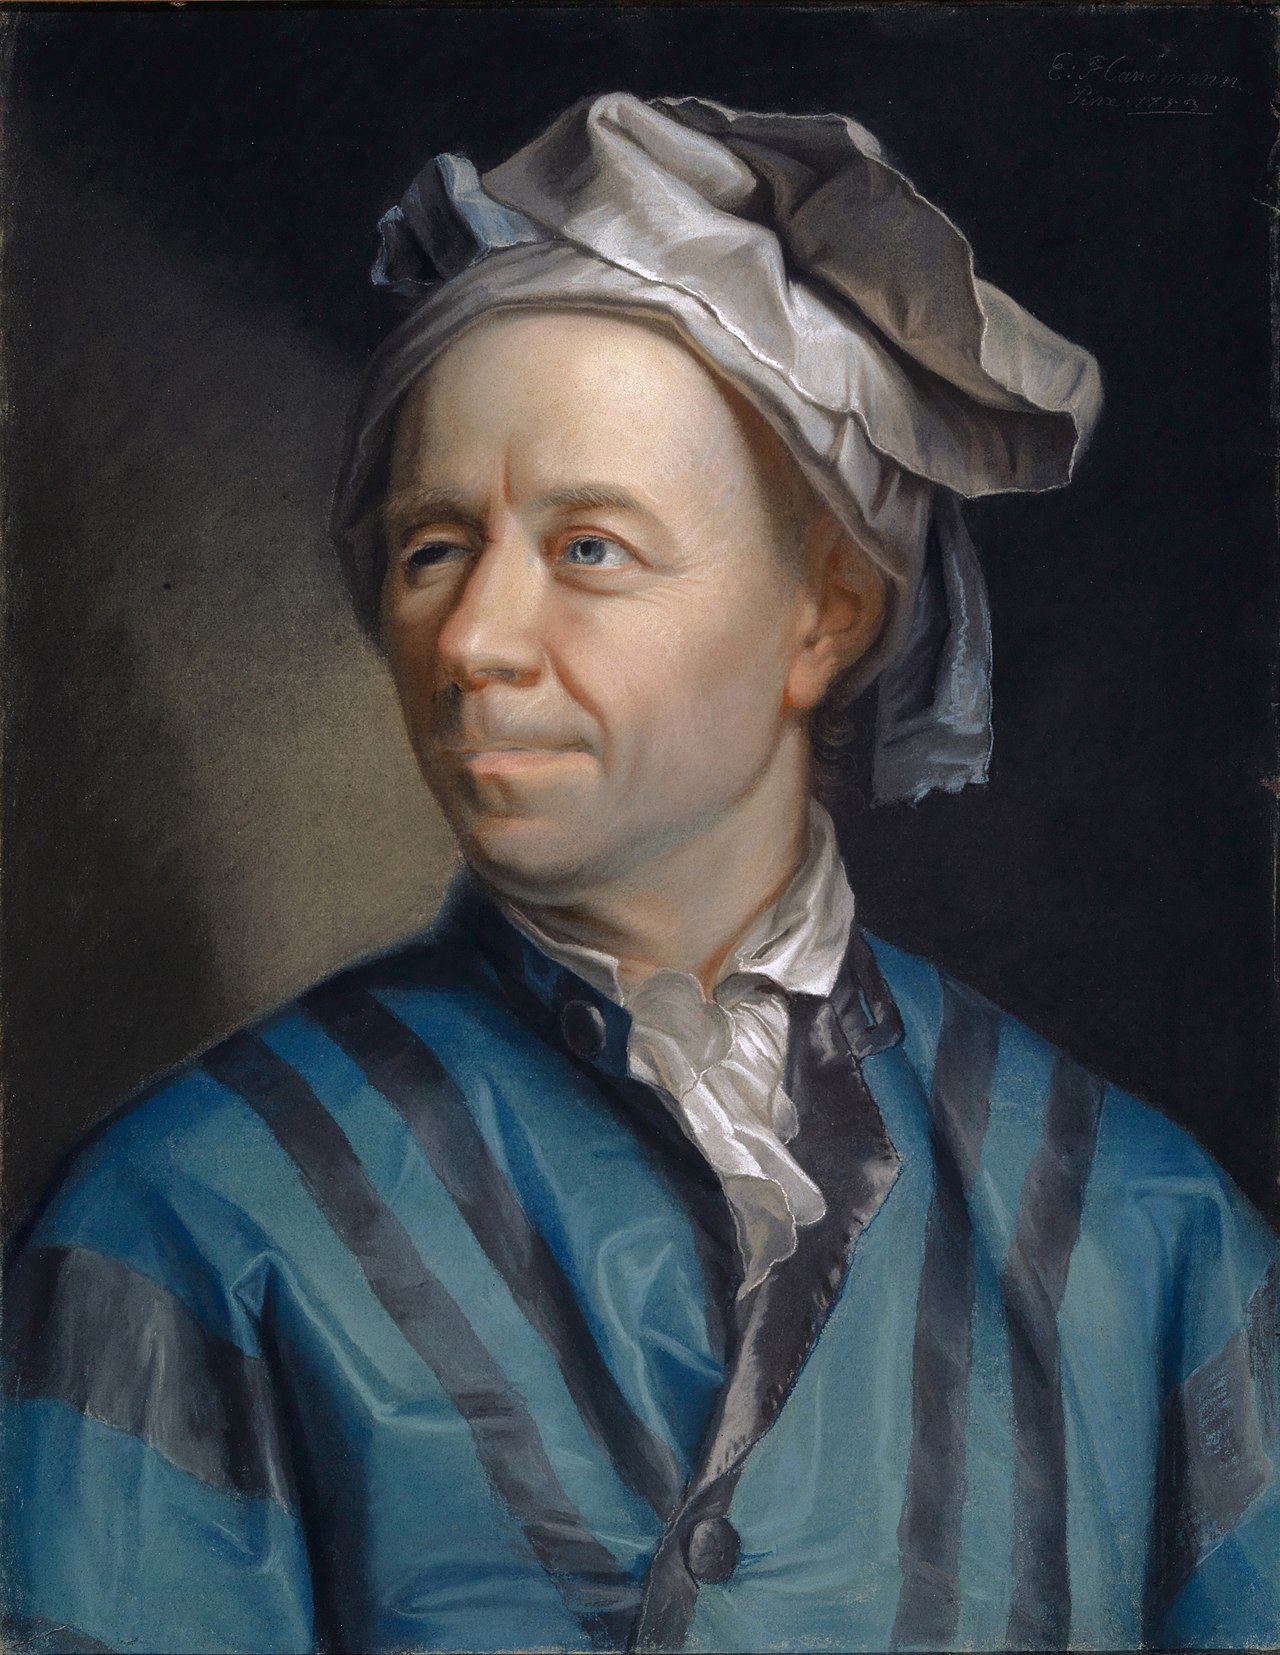
\includegraphics[height=0.23\textwidth]{./images/euler.jpg}\quad
        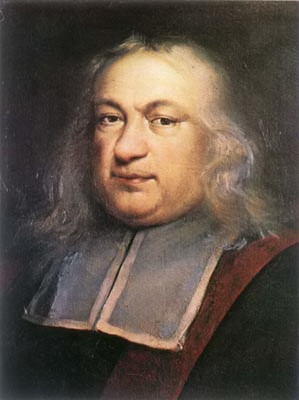
\includegraphics[height=0.23\textwidth]{./images/fermat.jpg}
        \caption{Leonhard Euler (1707--1783) and Pierre de Fermat (1607--1665)}\label{fig:euler}
\end{figure}
\subsection{Modular Exponentiation}

As shown in \S2, we must compute $a^n$ where both $a, n \in \mathbb{N}$
for SS . We could simply multiply:
\[
  a^n = \overbrace{a \times a \times \cdots \times a \times a}^n .
\]
The number of multiplications is $n-1$,
which is ${O}(n)$. While correct, this approach is na{\"{i}}ve and
\emph{extremely inefficient}. Since we are working with very large
numbers in SS, we must be able to compute modular exponentiation
quickly. So the question is, can we do better? We can in fact do much
better, computing $a^n$ in $\operatorname{O}(\log_2(n))$ steps.

Recall that we can write any integer as a polynomial
\[
  n = c_m 2^m + c_{m-1} 2^{m-1} + \cdots + c_1 2^1 + c_0 2^0 =
  \sum_{0\le i \le m} c_i 2^i ,
\]
where $n \ge 2^m$ and $c_i \in \{0, 1\}$. And so,
\[
  a^n = a^{c_m 2^m + c_{m-1} 2^{m-1} + \cdots + c_1 2^1 + c_0 2^0} .
\]
Since $a^{b+c} = a^b \times a^c$, then we can rewrite the formula as
\[
  a^n = a^{c_m 2^m} \times a^{c_{m-1} 2^{m-1}} \times \cdots \times
  a^{c_1 2^1} \times a^{c_0 2^0} = \prod_{0\le i \le m} a^{c_i 2^i} .
\]
As an example, consider $a^{13} = a^{2^3 + 2^2 + 2^0} = a^{8 + 4 + 1} =
a^8 \times a^4 \times a^1$. You will want to try a few more to get a
feeling for it before you attempt to write code.

This leaves us with the problem of computing the $a^{2^i}$ terms. We
start with $a = a^1$ and if we square it then $(a^1)^2 = a^2$. Each
time we square, $(a^2)^2 = a^4, (a^4)^2 = a^8, \ldots$ the exponents
are a power of $2$. We only have to square our previous result $\log_2
n$ times at most.

You will notice that the numbers get \emph{very large, very fast}.
Although we want enormous numbers for cryptography, we do not want
numbers that would be impossible to even write down if we used every
atom in the universe. Recall that $10^k$ is $k$ digits long. That
means that if $k=10^{1000}$ then there are that many digits (there are
approximately $10^{82}$ atoms in the observable universe).
Consequently, we will usually do such computations (mod ${n}$) for
some modulus $n$, meaning that all numbers are in $\{0, \ldots,
n-1\}$.

To implement modular exponentiation, you should simply follow the
steps to perform exponentiation by squaring as shown above and
reduce your results modulo $n$ after each operation that is likely to
yield a large result (you do not need to do it, if for example, you
just add a small constant). The following pseudocode shows the
repeated squaring and modular reduction at each step.

\begin{codebox}
  \Procname{\proc{Power-Mod}($a,d,n$)}
  \li $v \gets 1$
  \li $p \gets a$
  \li \While $d > 0$
  \li \Then \If \proc{Odd}(d)
  \li       \Then $v \gets (v \times p) \mod n$ \End
  \li       $p \gets (p \times p) \mod n$
  \li       $d \gets \lfloor d / 2 \rfloor$
      \End
  \li \Return $v$
\end{codebox}

The function that you are expected to implement to perform modular
exponentiation should be declared as follows:

\begin{funcdoc}{void pow\_mod(mpz\_t out, mpz\_t base, mpz\_t exponent,
  mpz\_t modulus)}
  Performs fast modular exponentiation, computing \texttt{base} raised
  to the \texttt{exponent} power modulo \texttt{modulus}, and storing
  the computed result in \texttt{out}.
\end{funcdoc}

\subsection{Primality Testing}
\epigraphwidth=0.6\textwidth
\epigraph{\emph{There are many methods---none of them as good as the randomized primality test.}}{---Michael O.\space Rabin, October 1997}


\noindent
The simplest primality test is trial division: given an input number,
$n$, check whether it is evenly divisible by any prime number between
$2$ and $\sqrt{n}$. Thus, this simple algorithm\footnote{
How big is $\sqrt{n}$? A typical encryption key has more than $600$ decimal digits. Thus,
$\sqrt{10^{600}}=10^{300}$.
Suppose we can do one trial division every \emph{nanosecond}, then that's $10^{300-9} = 10^{291}$ seconds. There are $22,896,000$ or about $10^7$ seconds per year, so it will take about $10^{284}$ years (the Big Bang was about $13.7\times 10^{9}$ years ago).
}
is $O(\sqrt{n})$,
but can we do better? The answer is subtle. To be certain,
we must try all of the primes from up to $\sqrt{n}$; there is no
way to escape it. But we can do much better if we are willing to
accept an answer of \emph{probably}.

Since it is infeasible to use a \emph{deterministic} algorithm, we
can solve many problems with \emph{high probability} by using a
\emph{randomized algorithm}. Such algorithms explore random parts
of the problem space so that we have high (but not perfect) confidence
that they have solved the problem.

Probabilistic tests are more rigorous than heuristic tests in that
they provide provable bounds on the probability of being fooled by
a composite number. All practical primality tests are probabilistic
tests. These tests use, apart from the tested number $n$, some other
number $a$ (called a \emph{witness}) that is chosen at random from
some sample space. The usual randomized primality tests never report
a prime number as composite, but a composite number may be reported
as prime.

The simplest probabilistic primality test is the Fermat primality
test. It works as follows: Given an integer $n$, choose some integer
a coprime to $n$ and calculate $a^{n - 1} \pmod{n}$. If the result
is different from $1$, then $n$ is composite. If it is $1$, then
$n$ may be prime. If $a^{n-1} \equiv 1 \pmod{n}$ $n$ is not prime,
then $n$ is called a pseudoprime to base $a$. In practice, we
observe that, if $a^{n-1} \equiv 1 \pmod{n}$, then $n$ is usually
prime.

Better yet is the Solovay-Strassen probabilistic primality test,
developed by Robert M.\xspace Solovay and Volker Strassen in 1977.
It is of particular importance since it made practical public-key
algorithms such as SS.

\begin{figure}[tbhp]
\centering
  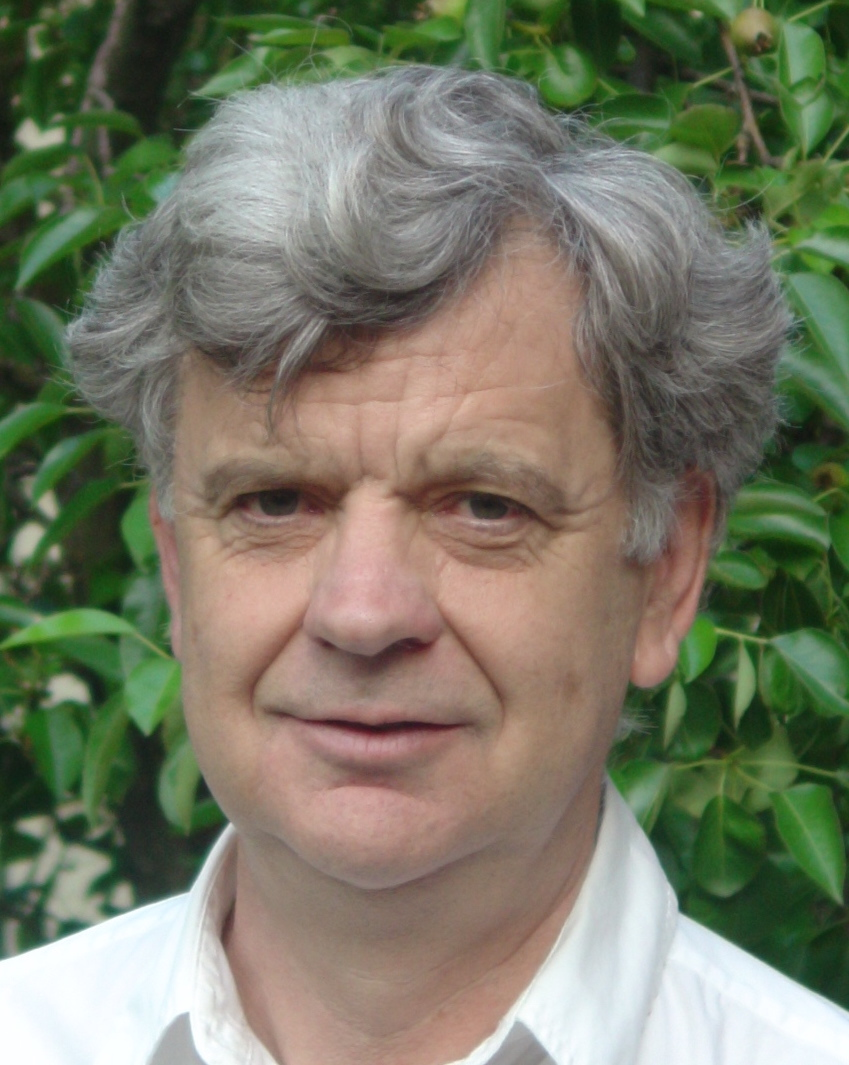
\includegraphics[height=0.33\textwidth]{./images/miller.jpg}\quad
  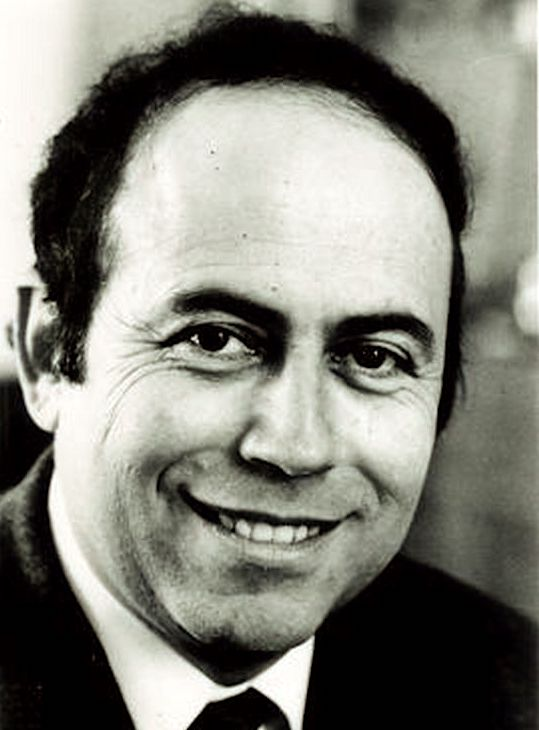
\includegraphics[height=0.33\textwidth]{./images/rabin.jpg}
\caption{Gary L.\xspace Miller and Michael O.\xspace Rabin}\label{fig:rabin}
\end{figure}

The Miller–Rabin primality test, invented by Gary Miller and Michael
O.\xspace Rabin (Figure\xspace\ref{fig:rabin}), is an even more
sophisticated probabilistic test, which detect all composites (once
again, this means: for every composite number $n$, at least
$\frac{3}{4}$ of numbers $a$ are witnesses of compositeness of $n$). The
accuracy of these tests is compared in Figure\xspace\ref{fig:tests}.

\begin{figure}[tbhp]
\centering
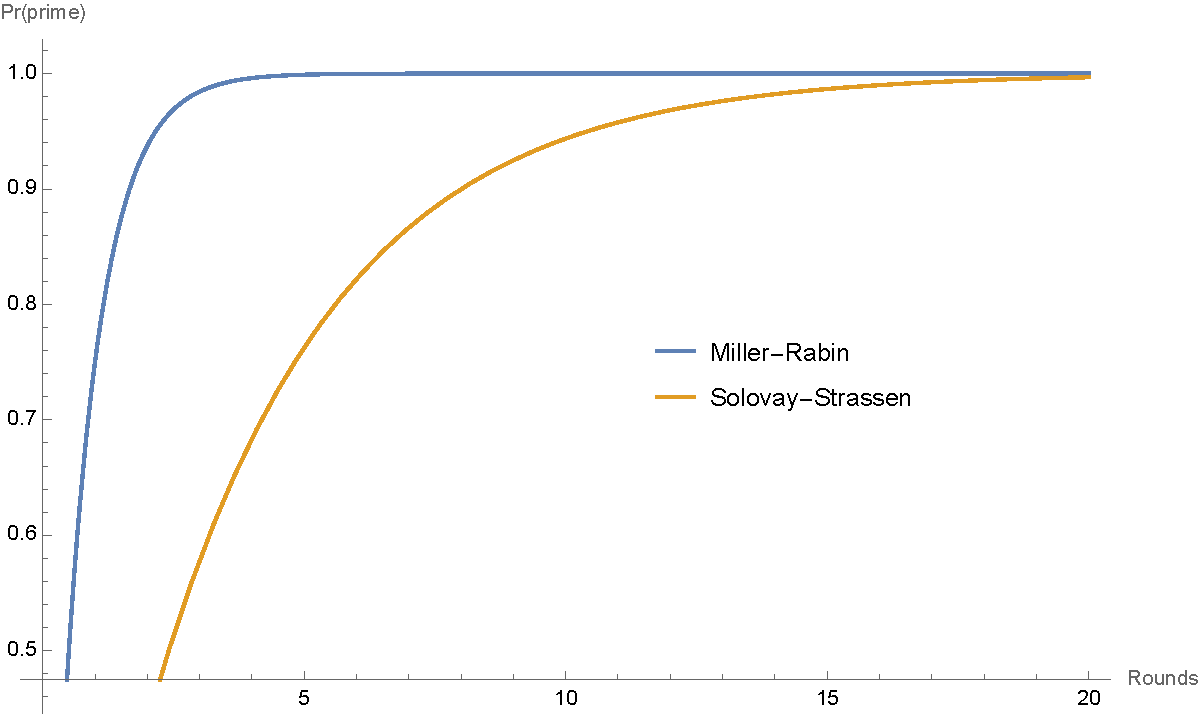
\includegraphics[width=0.75\textwidth]{./graphs/PrimeTest.pdf}
\caption{$\Pr[\text{prime}(p)]$ after successfully passing a given number of rounds.}\label{fig:tests}
\end{figure}

The Miller–Rabin primality test works as follows: Given an integer $n$,
choose some positive integer $a < n$. Let $2^s d = n - 1$, where $d$ is
odd. If $a^d \not\equiv \pm 1 \pmod{n}$ and $a^{{2^r} d} \not\equiv \pm
1 \pmod{n}$ for all $0 \le r \le s - 1$, then $n$ is composite and $a$
is a witness for the compositeness. Otherwise, $n$ \emph{might} be
prime. That is, we might be wrong $\frac{1}{4}$ of the time. If we
repeat the test $100$ times then our chance of being wrong is
$(\frac{1}{4})^{100} = 2^{-200}$ and that is usually more than good
enough. The Miller–Rabin test is considered a strong pseudoprime test,
where a pseudoprime is a number that is determined to be \emph{probably
prime} by a probabilistic test, but not actually prime. Deterministic
primality tests, such as the AKS primality test, do not give false
positives.

\begin{codebox}
  \Procname{\proc{Miller-Rabin}($n,k$)}
  \li write $n - 1 = 2^sr$ such that $r$ is odd
  \li \For $i \gets 1$ \To $k$
  \li \Then choose random $a \in \{\,2,3,\dots,n-2\,\}$
  \li       $y = \proc{Power-Mod}(a, r, n)$
  \li       \If $y \ne 1$ and $y \ne n - 1$
  \li       \Then $j \gets 1$
  \li             \While $j \le s - 1$ and $y \ne n - 1$
  \li             \Then $y \gets \proc{Power-Mod}(y, 2, n)$
  \li                   \If $y == 1$ \li \Then \Return \const{false} \End
  \li                   $j \gets j + 1$
                  \End
  \li             \If $y \ne n - 1$ \li \Then \Return \const{false} \End
            \End
      \End
  \li \Return \const{true}
\end{codebox}

The function that you are expected to implement to perform primality
testing should be declared as follows:

\begin{funcdoc}{bool is\_prime(mpz\_t n, uint64\_t iters)}
  Conducts the Miller-Rabin primality test to indicate whether or not
  \texttt{n} is prime using \texttt{iters} number of Miller-Rabin
  iterations. This function is needed when creating the two large primes
  $p$ and $q$ in SS, verifying if a large integer is a prime.
\end{funcdoc}

In addition to the \texttt{is\_prime()} function, you are also required
to implement the following function:

\begin{funcdoc}{void make\_prime(mpz\_t p, uint64\_t bits, uint64\_t
  iters)}
  Generates a new prime number stored in \texttt{p}. The generated prime
  should be at least \texttt{bits} number of bits long. The primality of
  the generated number should be tested using \texttt{is\_prime()} using
  \texttt{iters} number of iterations.
\end{funcdoc}

\subsection{Modular Inverses}

The Euclidean algorithm, also called  Euclid's algorithm, is an
efficient method for computing the greatest common divisor ($\gcd$) of
two integers, the largest number that divides them both with a zero
remainder. The Euclidean algorithm is based on the principle that the
greatest common divisor of two numbers does not change if their
difference replaces the larger number with the smaller number. Since
this replacement reduces the larger of the two numbers, repeating this
process gives successively smaller pairs of numbers until the two
numbers become equal. We can accomplish this much faster if we compute
the remainder, which is equivalent to subtracting the smaller number
from the larger until it is no longer larger. You will first want to
implement the following function to compute the greatest common divisor
of two integers, which should be defined as follows:

\begin{funcdoc}{void gcd(mpz\_t d, mpz\_t a, mpz\_t b)}
  Computes the greatest common divisor of \texttt{a} and \texttt{b},
  storing the value of the computed divisor in \texttt{d}.

  \begin{codebox}
    \Procname{\proc{gcd}($a,b$)}
    \li \While $b \ne 0$
    \li \Then $t \gets b$
    \li       $b \gets a \bmod b$
    \li       $a \gets t$
        \End
    \li \Return $a$
  \end{codebox}
\end{funcdoc}

The extended Euclidean algorithm is an extension to the Euclidean
algorithm, and computes, in addition to the greatest common divisor
(gcd) of integers a and b, also the coefficients of B\'ezout's identity,
which are integers $x$ and $y$ such that
\[
  a x + b y = \gcd(a, b) .
\]
The extended Euclidean algorithm is particularly useful when $a$ and $b$
are coprime. With that provision, $x$ is the modular multiplicative
inverse of $a \pmod{b}$, and $y$ is the modular multiplicative inverse
of $b \pmod{a}$.

B\'ezout's identity asserts that $a$ and $n$ are coprime if and only if
there exist integers $s$ and $t$ such that
\[
  n s + a t = 1.
\]
Reducing this identity modulo $n$ gives
\[
  a t \equiv 1 \pmod{n}.
\]
To adapt the extended Euclidean algorithm to the problem of computing
the multiplicative inverse, note that the B\'ezout coefficient of $n$ is
not needed and so does not need to be computed. Also, for getting a
positive and result that is less than $n$,  use the fact that the
integer $t$ provided by the algorithm satisfies $| t | < n$. That is, if
$t < 0$, add $n$ to it at the end.

\begin{codebox}
  \Procname{\proc{Mod-Inverse}($a,n$)}
  \li $(r, r') \gets (n, a)$
  \li $(t, t') \gets (0, 1)$
  \li \While $r' \ne 0$
  \li \Then $q \gets \lfloor r / r' \rfloor$
  \li       $(r, r') \gets (r', r - q \times r')$
  \li       $(t, t') \gets (t', t - q \times t')$
      \End
  \li \If $r > 1$ \li \Then \Return no inverse \End
  \li \If $t < 0$ \li \Then $t \gets t + n$ \End
  \li \Return $t$
\end{codebox}

The function that you are expected to implement to compute modular
inverses should be declared as follows:

\begin{funcdoc}{void mod\_inverse(mpz\_t i, mpz\_t a, mpz\_t n)}
  Computes the inverse \texttt{i} of \texttt{a} modulo \texttt{n}. In
  the event that a modular inverse cannot be found, set \texttt{i} to 0.
  Note that this pseudocode uses parallel assignments, which \textbf{C}
  \emph{does not} support. Thus, you will need to use auxiliary
  variables to fake the parallel assignments.
\end{funcdoc}
